\documentclass[12pt]{article}

\usepackage{amsmath,amsthm,amsfonts,amssymb,amsxtra}
\usepackage{pgf,tikz}
\usetikzlibrary{arrows}
\renewcommand{\theenumi}{(\alph{enumi})} 
\renewcommand{\labelenumi}{\theenumi}

\pagestyle{empty}
\setlength{\textwidth}{7in}
\setlength{\oddsidemargin}{-0.5in}
\setlength{\topmargin}{-1.0in}
\setlength{\textheight}{9.5in}

\theoremstyle{definition}
\newtheorem{problem}{Problem}

\begin{document}

\noindent{\large\bf MATH 241}\hfill{\large\bf Exam \#3}\hfill{\large\bf
  Spring 2017}\hfill{\large\bf Page 1/5}\hrule

\bigskip
\begin{center}
  \begin{tabular}{|ll|}
    \hline & \cr
    {\bf Name: } & \makebox[12cm]{\hrulefill}\cr & \cr
    {\bf VIP ID:} & \makebox[12cm]{\hrulefill}\cr & \cr
    \hline
  \end{tabular}
\end{center}
\begin{itemize}
\item Write your name and your VIP ID in the space provided above.
\item The test has five (5) pages, including this one.
\item Enter your answer in the box(es) provided.
\item You must show sufficient work to justify all answers unless
  otherwise stated in the problem.  Correct answers with inconsistent
  work may not be given credit.
\item Credit for each problem is given in parentheses at the right of
  the problem number.
\end{itemize}
\hrule

\begin{center}
  \begin{tabular}{|c|c|c|}
    \hline
    &&\cr
    {\large\bf Page} & {\large\bf Max.~points} & {\large\bf Your points} \cr
    &&\cr
    \hline
    &&\cr
    {\Large 2} & \Large 50 & \cr
    &&\cr
    \hline
    &&\cr
    {\Large 3} & \Large 50 & \cr
    &&\cr
    \hline\hline
    &&\cr
    {\large\bf Total} & \Large 100 & \cr
    &&\cr
    \hline
  \end{tabular}
\end{center}
\newpage

%%%%%%%%%%%%%%%%%%%%%%%%%%%%%%%%%%%%% Page 2
\noindent{\large\bf MATH 241}\hfill{\large\bf Exam \#3}\hfill{\large\bf
  Spring 2017}\hfill{\large\bf Page 2/5}\hrule

\bigskip
\begin{problem}[20 pts---10 points each] Find equations of the tangent plane to the graph of the following functions at the indicated points.
\begin{enumerate}
  \item $f(x,y) = \sqrt{x^2+y}$ at $P=(0,1,1)$.
  \vspace{1cm}
  \begin{flushright}
  \begin{tikzpicture}
    \draw (-4.8cm, 0.5cm) node {Plane:};
    \draw (-4cm, 0cm) rectangle (5cm,1cm);
  \end{tikzpicture}
  \end{flushright}
  \item $f(x,y) = x\sin(xy)$ at $P=\big(1,\frac{\pi}{2},1 \big)$
  \vspace{1cm}
  \begin{flushright}
  \begin{tikzpicture}
    \draw (-4.8cm, 0.5cm) node {Plane:};
    \draw (-4cm, 0cm) rectangle (5cm,1cm);
  \end{tikzpicture}
  \end{flushright}
\end{enumerate}
\end{problem}
\hrule

\begin{problem}[10 pts]
Find the direction in which the function $f(x,y)= x^2 + y^2$ increases more rapidly at the point $(1,1)$.  What is that value?

\vspace{2cm}
\begin{flushright}
  \begin{tikzpicture}
    \draw (3cm, 0.5cm) node {Value:};
    \draw (4cm, 0cm) rectangle (10cm,1cm);
    \draw (-5cm, 0.5cm) node {Direction:};
    \draw (-4cm, 0cm) rectangle (2cm,1cm);
  \end{tikzpicture}
  \end{flushright}
\end{problem}
\hrule

\begin{problem}[20 pts]
Find and classify all the critical points of the function 
\begin{equation*}
f(x,y) = 3y^2 - 2y^3-3x^2+6xy.
\end{equation*}
\end{problem}

\newpage

%%%%%%%%%%%%%%%%%%%%%%%%%%%%%%%%%%%%% Page 3
\noindent{\large\bf MATH 241}\hfill{\large\bf Exam \#3}\hfill{\large\bf
  Spring 2017}\hfill{\large\bf Page 3/5}\hrule

\bigskip
\begin{problem}[50 pts---10 pts each part]
Find the absolute maximum and minimum values of the function $f(x,y) = 4x+6y-x^2-y^2+7$ on the set $D = \big\{ (x,y) : 0 \leq x \leq 4, 0 \leq y \leq 5 \big\}$.  

I will walk you through the different steps:
\begin{enumerate}
\item Sketch the domain $D$.

\begin{tikzpicture}[scale=0.7]
\draw [white] (-0.5,-0.5) rectangle (6.5,6.5);
\draw [<->, ultra thick] (-0.5,0) -- (6.5,0);
\draw [<->, ultra thick] (0,-0.5) -- (0,6.5);
\draw[step=0.5,gray,ultra thin] (-0.25, -0.25) grid (6.25, 6.25);
\end{tikzpicture}
\item Let's gather some candidates.  The first kind of candidates are the critical points of $f$.  Find them.  For those on the domain $D$, place them in the diagram above, and indicate the value of the function in those locations.

\vspace{2cm}
\item The rest of candidates are going to be located on the border of the domain $D$.  Find first parametric equations for each of the curves that define the border of $D$.  Do that work on page 4.  Label them accordingly in the diagram above.

\vspace{2.5cm}
\item On each of the curves that define the border of $D$, find candidates for absolute maximum and absolute minimum.  Do the work on page 5, and report those points (with their values) here.
\begin{center}
\begin{tabular}{ll}
Candidates for Maxima  & Candidates for Minima \\
\begin{tabular}{|c|c|}
\hline Point(s) & value \\
\hline \hspace{4cm} & \hspace{1.5cm} \\ 
\hline & \\ 
\hline & \\ 
\hline & \\ 
\hline & \\ 
\hline
\end{tabular} &
\begin{tabular}{|c|c|}
\hline Point(s) & value \\
\hline \hspace{4cm} & \hspace{1.5cm} \\ 
\hline & \\ 
\hline & \\ 
\hline & \\ 
\hline & \\ 
\hline
\end{tabular}
\end{tabular}
\end{center}
\item Where are the absolute maxima and minima of $f$ on $D$?  What are their values?
\begin{flushright}
  \begin{tikzpicture}
    \draw (-12cm, 0.5cm) node {max:};
    \draw (-11.4cm,-0cm) rectangle (-4.5cm,1cm);
    \draw (-3.6cm, 0.5cm) node {min:};
    \draw (-3cm, 0cm) rectangle (4cm,1cm);
  \end{tikzpicture}
\end{flushright}
\end{enumerate}
\end{problem}

\newpage

%%%%%%%%%%%%%%%%%%%%%%%%%%%%%%%%%%%%% Page 4
\noindent{\large\bf MATH 241}\hfill{\large\bf Exam \#3}\hfill{\large\bf
  Spring 2017}\hfill{\large\bf Page 4/5}\hrule

\bigskip
{\Large Scratch paper for part (c) of Problem 1.}
\newpage

%%%%%%%%%%%%%%%%%%%%%%%%%%%%%%%%%%%%% Page 5
\noindent{\large\bf MATH 241}\hfill{\large\bf Exam \#3}\hfill{\large\bf
  Spring 2017}\hfill{\large\bf Page 5/5}\hrule

\bigskip
{\Large Scratch paper for part (d) of Problem 1.}


\end{document}
